\section{Run 1}

As first approach we had to develop a classifier which use as features \textit{tiny images}. This particular representation consists on few simple steps: initially we resize the image to a 16x16 matrix, then we build a vector of 256 pixels composed of the consecutive rows of the new image. 

After that, in order to improve classification performances, we implemented two different types of normalization to the vector, which in the following we refer to as \textbf{x}:
\begin{itemize}
	\item \textbf{standard normalization}: $\mathbf{\bar{x}} = \frac{\mathbf{x} - \mu}{\sigma}$ where $\mu$ is the mean of \textbf{x} and $\sigma$ is its standard deviation
	\item \textbf{unit length normalization}: $\mathbf{\widehat{x}} = \frac{\mathbf{\bar{x}}}{\left \| \mathbf{\bar{x}} \right \|}$
\end{itemize} 
In this way we obtained a set of unit length vectors of zero mean.

The idea behind the classifier is that one vector representing an image of a specific class will likely be similar to other vectors of the same category. So, once we perform this operation for all the training set, we can determine the category of each image of the validation set using the \textbf{k-nearest-neighbour} classifier: this means that we evaluate the distance between the tiny image to validate and all the vectors from the training set; then, we pick the k nearest vectors (of which we know the class) and we classify our image with the most represented class in the neighbourhood. In case we have two classes most represented we can implement different choice polices, in our case we used the first classes returned by MATLAB.

In order to find better performances, we tried to tune the value of k for the several measures of distance available in \code{vl\_alldist2}, in particular:

\begin{equation}
	\mathbf{L_{INF}}=  max|X - Y| \qquad
	\mathbf{L_2}= sum(X - Y)^2 \qquad
	\mathbf{L_1}= sum|X - Y|
\end{equation} 
\begin{figure}[h]
	\centering
		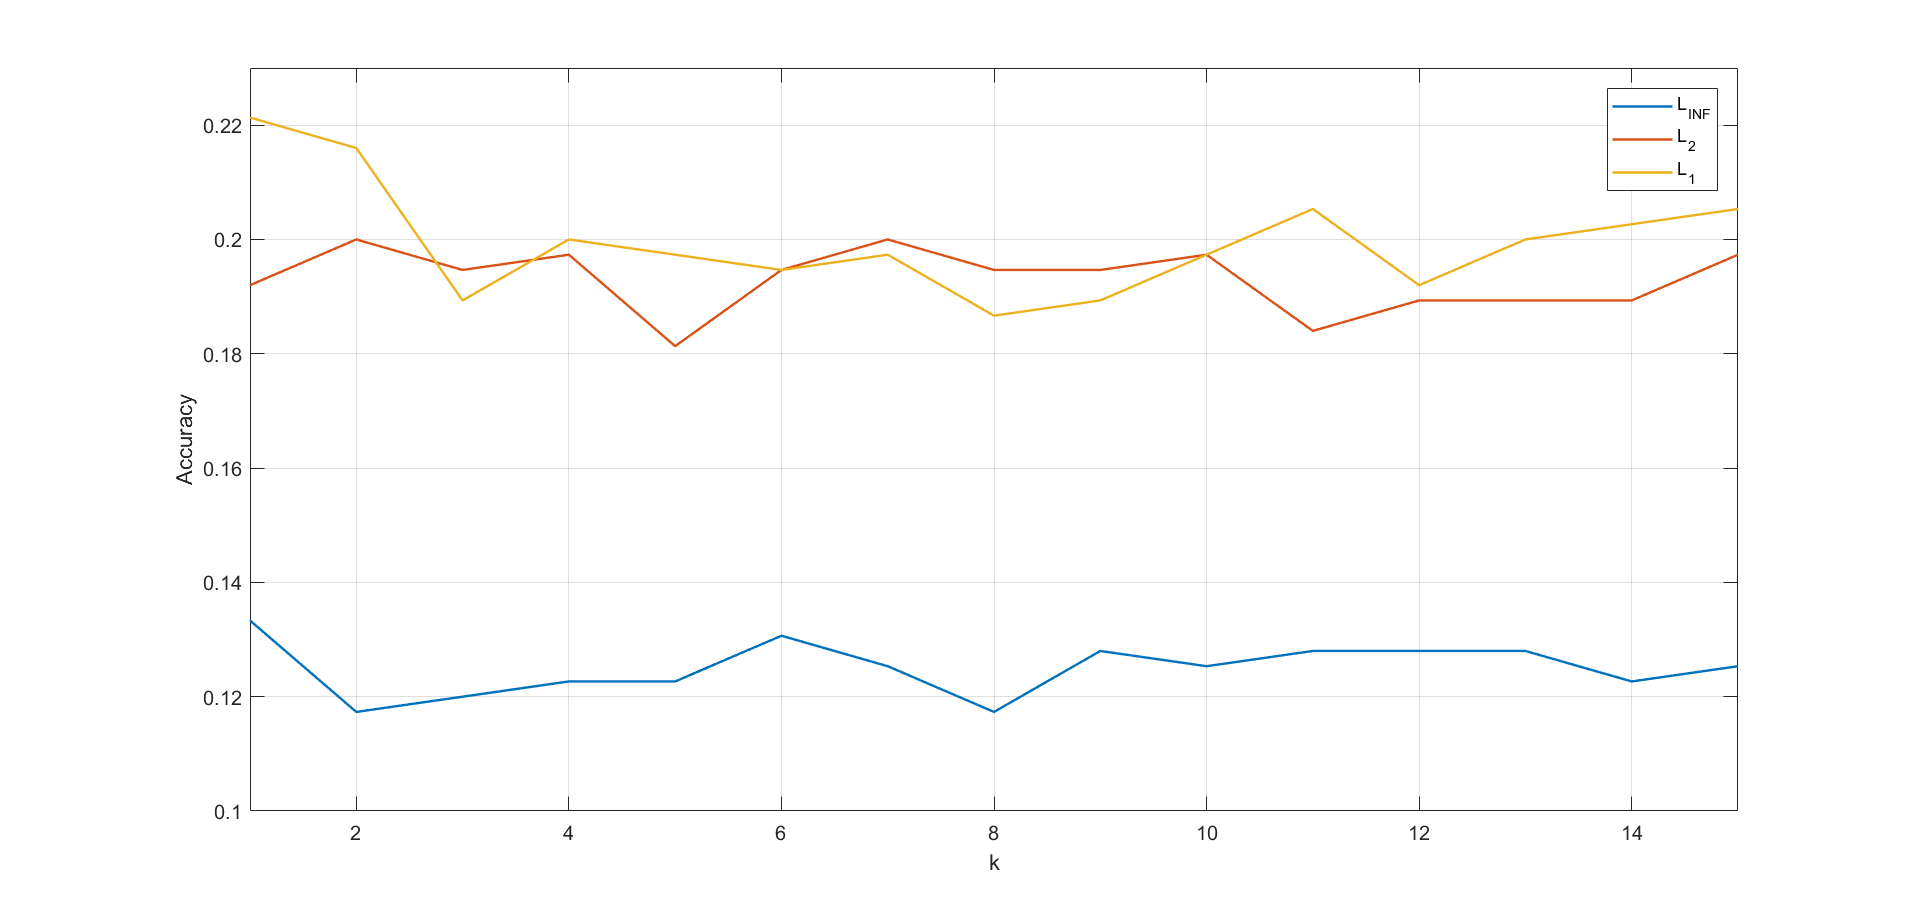
\includegraphics[height=.35\linewidth]{img/kaccuracy}
	\caption{Performances of different distance measures in function of k }
	\label{fig_kaccuracy}
\end{figure}

As we can see from Figure \ref{fig_kaccuracy}, while $L_{INF}$ can't reach even the 14\% of accuracy, $L_2$ and $L_1$ can reach up to 20\% and beyond. It's interesting to highlight that the latter perform better when we use either just the nearest neighbour or we increase the number of neighbours beyond 10, while $L_2$ presents its maximum around 7 or 8.
In conclusion, considering its stable behaviour on different runs that we performed, we decided to implement our classification using $L_2$ with k = 7. Of course, given the simplicity of these features, we couldn't expect more than 20\% of accuracy. On the following sections we will implement different features extraction methods to improve these performances.